\section{Présentation du logiciel}

\subsection{Fonctionnement du jeu et contraintes}
Pour décider de l'implémentation de notre logiciel, il convient bien sûr d'en cerner les mécanismes, et les interactions avec l'utilisateur. Nous les avons donc formalisé au moyen de différents diagrammes.

\subsubsection{Cas d'utilisations}
Sur les diagrammes de cas d'utilisations, on voit les différentes interactions possibles entre le logiciel et le joueur. Sur la figure \ref{casdut1}, on regroupe les interactions possibles avec le menu du logiciel, avant la partie. 

\begin{figure}[!h] 
\centerline{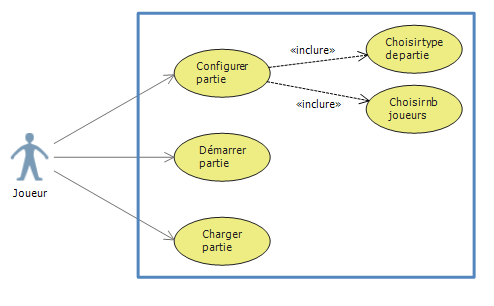
\includegraphics[width=\textwidth]{img/ucd_ihm_menus.png}}
   \caption{\label{étiquette} Diagramme de cas d'utilisations global}
\label{casdut1}
\end{figure}

Sur ce diagramme de cas d'utilisation, on présente les interactions possibles en jeu : manipulations d'unités etc ...
\begin{figure}
	\centering
		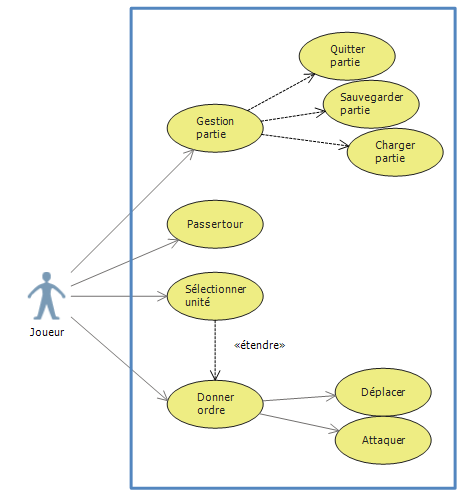
\includegraphics[width=\textwidth]{img/ucd_ig.png}
		 \caption{\label{étiquette} Diagramme de cas d'utilisations en jeu}
	\label{casdut2}
\end{figure}

\subsubsection{Déroulement d'une partie}
Nous avons illustré le fonctionnement d'une partie grâce à un diagramme d'activité. Il ets basé sur le fait qu'il n'y ait que deux joueurs (élément du cahier des charges), même si l'étendre ne changerait que peu de choses.
\begin{figure}[!h] 
\centerline{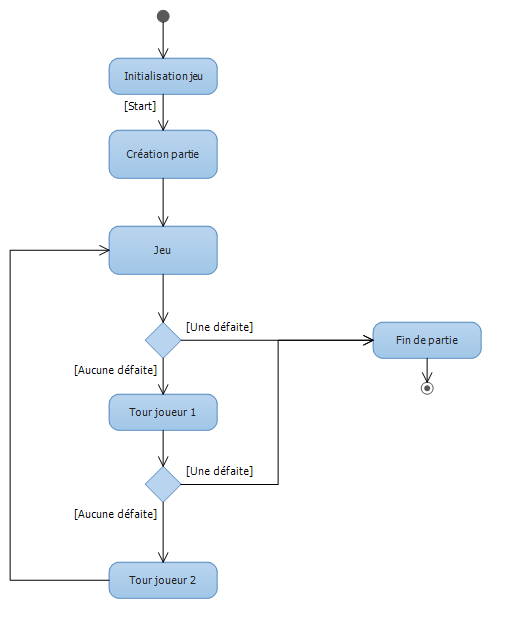
\includegraphics[width=\textwidth]{img/activite_jeu_ex.png}}
   \caption{\label{étiquette} Diagramme d'activité représentant le déroulement d'une partie pour deux joueurs}
\label{activiteTour}
\end{figure}

\subsubsection{Déroulement d'un tour}
Le joueur pouvant exécuter de nombreuses actions lors de son tour, nous avons voulu détailler le déroulement d'un tour lambda pour un joueur. Ainsi, nous avons tout d'abord fait un diagramme d'activité permettant une bonne visualisation d'ensemble du tour. On peut voir toutes les actions réalisables, combien de fois le joueur peut les éxecuter, et quelles sont les conditions pour terminer son tour. Le diagramme est représenté sur la figure \ref{activiteTour}

\begin{figure}[!h] 
\centerline{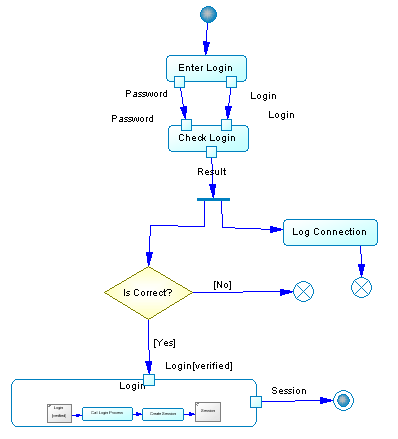
\includegraphics[width=\textwidth]{img/activite_tour_ex.png}}
   \caption{\label{étiquette} Diagramme d'activité représentant le déroulement d'un tour pour un joueur}
\label{activiteTour}
\end{figure}

Ensuite, afin d'avoir une vision du tour et des actions du joueur mais en terme de méthodes, de classes et d'interactions, nous avons fait un diagramme de séquence. Il représente le tour d'un joueur ou celui-ci décide de déplacer une de ses unités, puis de terminer son tour. Ce diagramme est représenté sur la figure \ref{sequenceTour}.\\

\begin{figure}[!h] 
\centerline{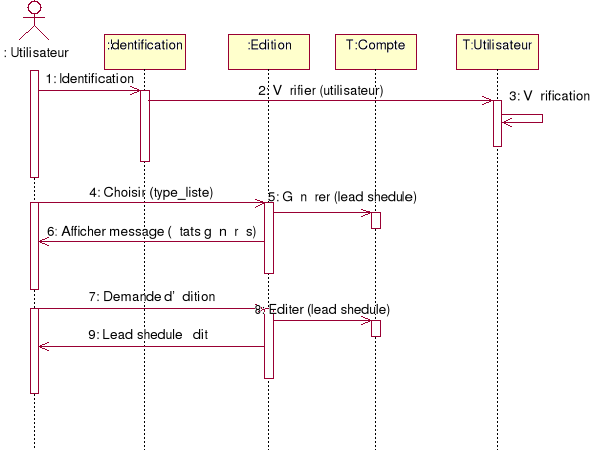
\includegraphics[width=\textwidth]{img/sequence_tour_ex.png}}
   \caption{\label{étiquette} Diagramme de séquence représentant le déroulement d'un tour pour un joueur}
\label{sequenceTour}
\end{figure}

\subsection{Déroulement d'une partie}
Après avoir développé un seul tour, nous nous sommes demandés l'interaction entre les tours des joueurs jusqu'à la victoire de l'un d'entre eux. Comme pour le cas d'un seul tour, nous trouvons que les diagrammes de séquences de sont pas adaptés à avoir une vue d'ensemble facilement compréhensible d'un système, c'est pourquoi nous avons fait un autre diagramme d'activité. Il permet de mieux comprendre le fonctionnement d'un tour. Il est représenté en figure \ref{activiteJeu}.\\

\begin{figure}[!h] 
\centerline{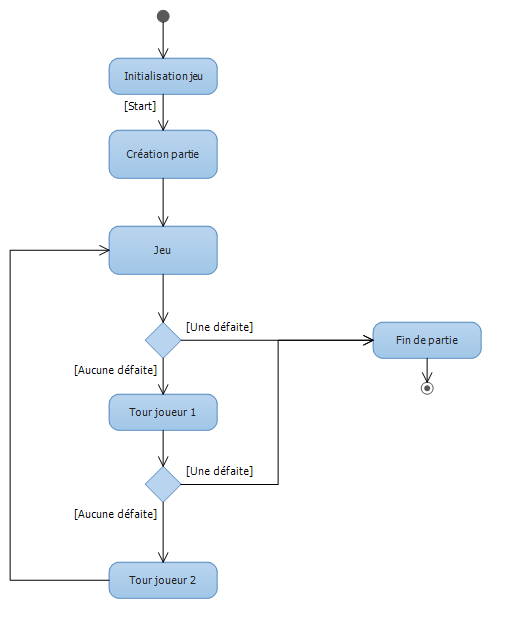
\includegraphics[width=\textwidth]{img/activite_jeu_ex.png}}
   \caption{\label{étiquette} Diagramme d'activité représentant le déroulement d'un tour pour un joueur}
\label{activiteJeu}
\end{figure}

Nous avons complété ce diagramme d'activité par un diagramme de séquence, réprésenté en figure \ref{sequenceJeu}, explicitant une partie standard avec des "blocs" comme play(), qui se réfèrent au diagramme de séquence précédent.  

\begin{figure}[!h] 
\centerline{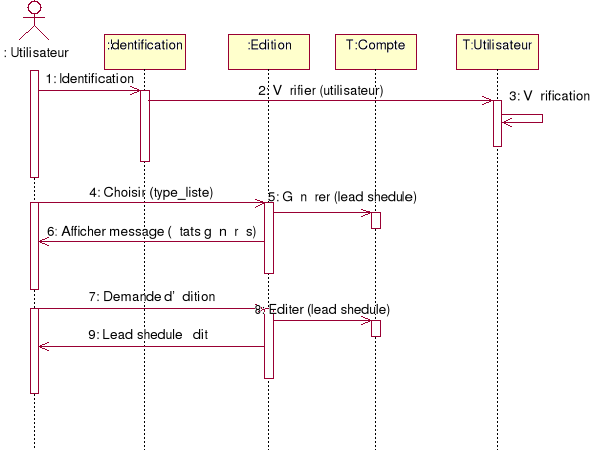
\includegraphics[width=\textwidth]{img/sequence_jeu_ex.png}}
   \caption{\label{étiquette} Diagramme de séquence représentant le déroulement d'un tour pour un joueur}
\label{sequenceJeu}
\end{figure}

\subsection{Architecture générale}
Notre analyse porte sur l'architecture générale du logiciel. Nous avons conçu un diagramme de classe correspondant à notre vision du jeu, basé sur les résultats d'analyse précédents. Celui ci étant plutôt chargé, il est scindé en plusieurs diagramme pour chaque grande partie.

\subsubsection{Interactions entre les objets
Pour produire le code le plus générique possible, nous organisons les objets en classes abstraite qui implémentent des interfaces. De ces classes abstraite, hériteront des classes qui correspondent aux objets du jeu.
}
\begin{figure}[!h] 
\centerline{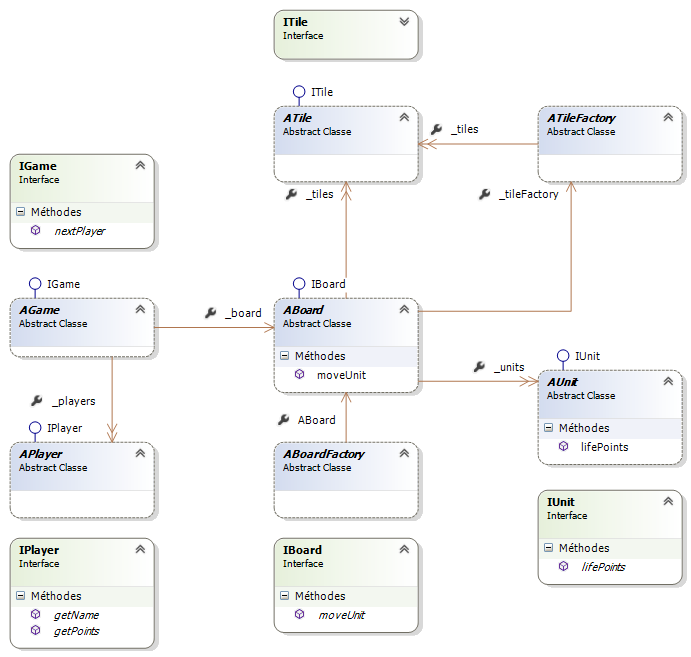
\includegraphics[width=\textwidth]{img/cd_interactions_between_class.png}}
   \caption{\label{étiquette} Diagramme de classe : Interactions entre objets}
\label{inter_bet_class}
\end{figure}

Le prochain diagramme résume quelles classes héritent des classes abstraites précédemment définies.
\begin{figure}[!h] 
\centerline{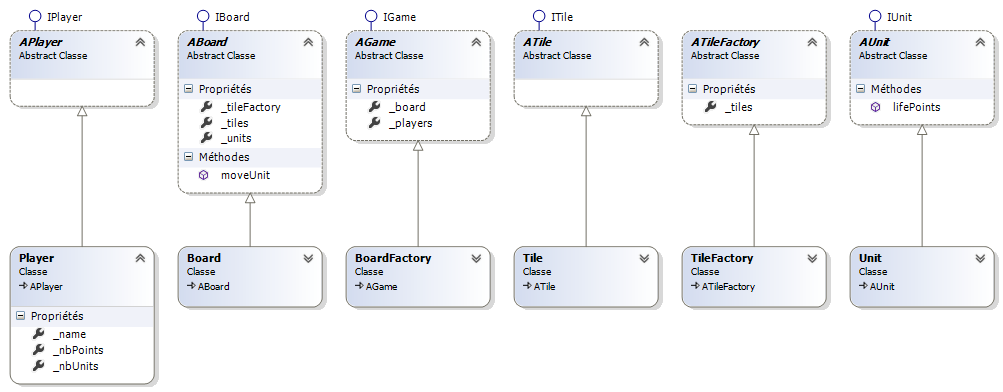
\includegraphics[width=\textwidth]{img/cd_inter_with_abstract.png}}
   \caption{\label{étiquette} Diagramme de classe : Interactions entre objets}
\label{inter_with_abstract}
\end{figure}

Sur ce diagramme, nous avons 5 principaux acteurs.\\
\begin{itemize}
  \item Le Jeu, ou Game, qui représente la partie du jeu. Il fait le lien entre le Joueur (Player) et le Plateau (Board). Il en existe plusieurs type : un jeu tout juste créé, et un jeu sauvegardé. Il respecte la stratégie monteur.
	
	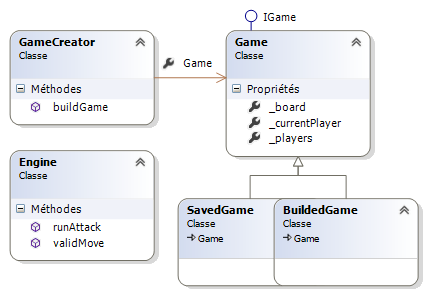
\includegraphics[width=\textwidth]{img/cd_game.png}
	
  \item Le Joueur, ou Player, est la classe représentant, comme son nom l'indique, le joueur. C'est lui qui va interagir avec la vue du plateau, et qui donnera des ordres à ses Unités.
		
  \item Le Plateau, ou Board, contient les cases sur lequel le jeu évolue. Il contient aussi les différentes unités en jeu. Cela permet un accès plus rapide pour le traitement de certaines actions.
	
	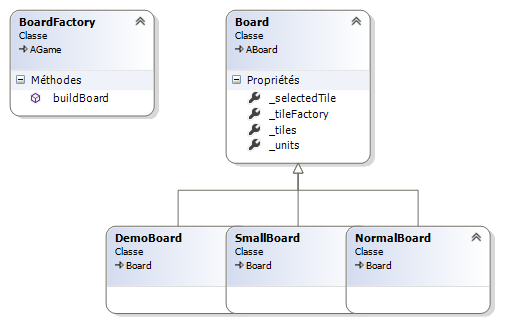
\includegraphics[width=\textwidth]{img/cd_board.png}
	
  \item Les Cases, ou Tiles, sont les cases, au sens individuel du terme, contenues sur le Plateau. Elle possèdent les Unités qui se trouvent sur elle. Elle hérite 4 autres classes, chacune correspondant au type de terrain associé : Plaine, Désert, Forêt, Montagne.
	
	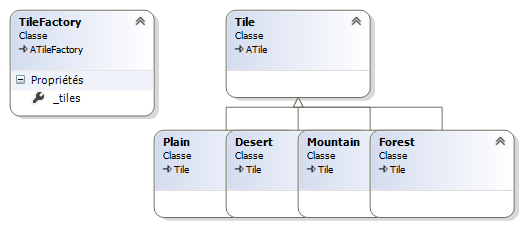
\includegraphics[width=\textwidth]{img/cd_tiles.png}
	
  \item Les Unités, ou Units, sont les personnages évoluant sur la carte. Les différents peuple sont ici défini comme héritant la classe Unité. Ainsi, on peut surcharger des fonctions, comme le déplacement ou l'attaque, en fonction du peuple de l'Unité : Elf, Orc ou Nain.
	
	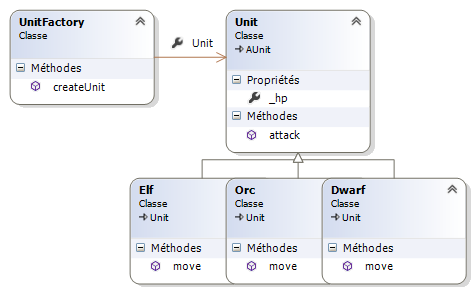
\includegraphics[width=\textwidth]{img/cd_units.png}
	
\end{itemize}

\newpage
